\documentclass[tikz,border=0pt,11pt]{standalone}
\usepackage[T1]{fontenc}
\usepackage[utf8]{inputenc}
\usepackage{lmodern,amsmath,amssymb}
\usepackage[swedish]{babel}
\usetikzlibrary{arrows.meta,calc,positioning,decorations.pathmorphing,decorations.pathreplacing,patterns,shadings}
\definecolor{navy}{HTML}{102F40}
\definecolor{teal}{HTML}{147D78}
\definecolor{lightteal}{HTML}{E6F1ED}
\definecolor{gold}{HTML}{B88B3B}
\definecolor{palegold}{HTML}{F7EEDB}
\definecolor{rust}{HTML}{B6533B}
\definecolor{palerust}{HTML}{FAEAE4}
\definecolor{paper}{HTML}{F7F5EE}
\definecolor{muted}{HTML}{5B6D72}
\definecolor{line}{HTML}{D6DED8}
\renewcommand{\familydefault}{\sfdefault}
\newcommand{\atom}[5]{\shade[ball color=#3!70] (#1,#2) circle (#5);\node[text=white,font=\bfseries\small] at (#1,#2){#4};}
\newcommand{\water}[3]{\begin{scope}[shift={(#1,#2)},scale=#3]\draw[navy!45,line width=2pt] (-.3,.22)--(0,0)--(.3,.22);\atom{0}{0}{rust}{O}{.22}\atom{-.3}{.22}{teal}{H}{.15}\atom{.3}{.22}{teal}{H}{.15}\end{scope}}
\newcommand{\panel}[4]{\filldraw[fill=white,draw=line,rounded corners=5pt] (#1,#2) rectangle ++(#3,#4);}
\newcommand{\note}[4]{\node[txt,text width=#3cm] at (#1,#2){#4};}
\tikzset{txt/.style={anchor=north west,align=left,text=navy,font=\small},
 head/.style={anchor=west,text=navy,font=\bfseries\large},
 label/.style={align=center,text=navy,font=\small},
 smalllabel/.style={align=center,text=muted,font=\footnotesize},
 arrow/.style={-{Latex[length=2.5mm,width=1.8mm]},line width=1.2pt,draw=teal},
 goldarrow/.style={-{Latex[length=2.5mm]},line width=1.2pt,draw=gold},
 rustarrow/.style={-{Latex[length=2.5mm]},line width=1.2pt,draw=rust},
 dashedarrow/.style={arrow,dashed},
 badge/.style={fill=lightteal,rounded corners=3pt,text=teal,font=\bfseries\small,inner sep=5pt}}
\begin{document}
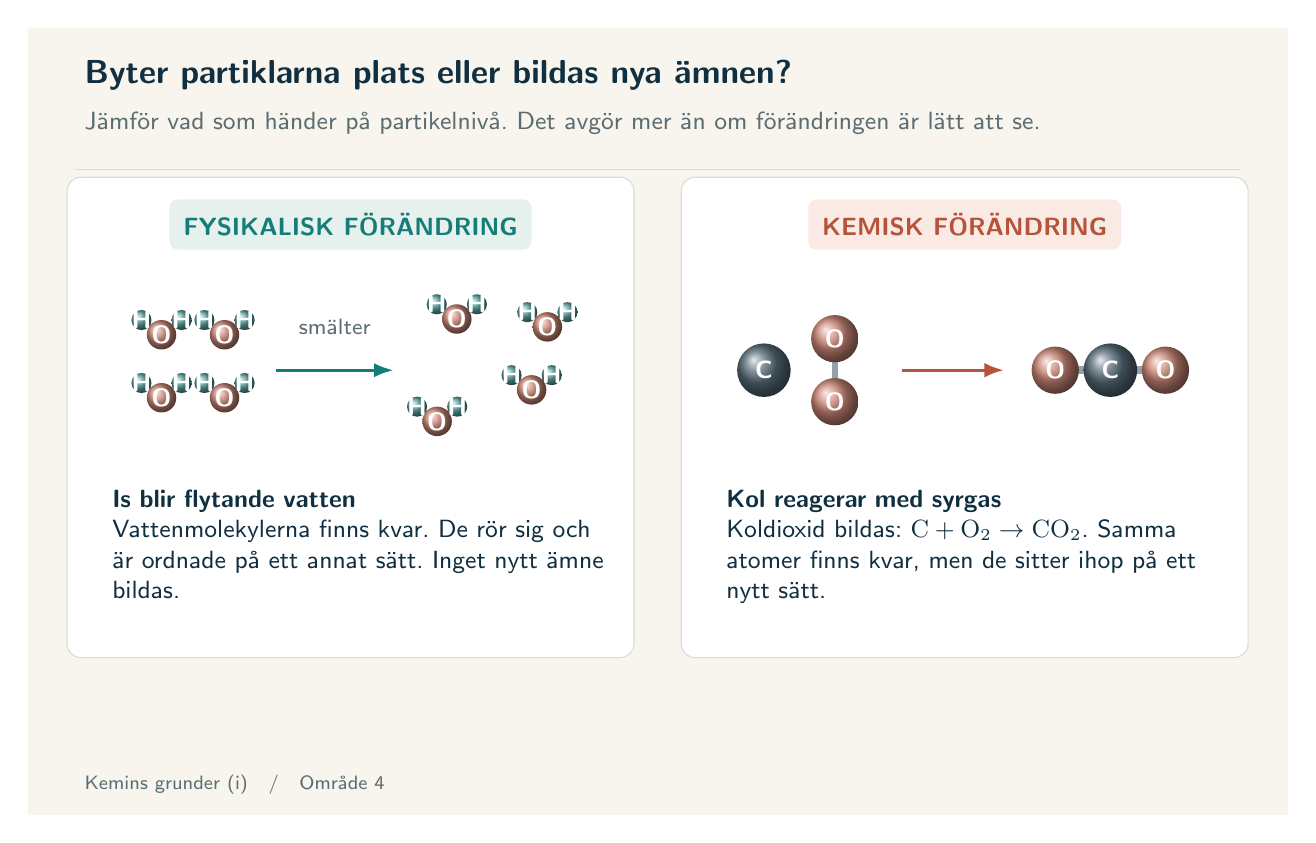
\begin{tikzpicture}[x=1cm,y=1cm]
\path[use as bounding box] (0,0) rectangle (16,10);
\fill[paper] (0,0) rectangle (16,10);
\node[head] at (.6,9.4){Byter partiklarna plats eller bildas nya ämnen?};
\note{.6}{9.05}{14.8}{\textcolor{muted}{Jämför vad som händer på partikelnivå. Det avgör mer än om förändringen är lätt att se.}}
\draw[line] (.6,8.2)--(15.4,8.2);

\panel{.5}{2}{7.2}{6.1}\panel{8.3}{2}{7.2}{6.1}
\node[badge] at (4.1,7.5){FYSIKALISK FÖRÄNDRING};\node[badge,fill=palerust,text=rust] at (11.9,7.5){KEMISK FÖRÄNDRING};
\foreach \x/\y in {1.7/5.3,2.5/5.3,1.7/6.1,2.5/6.1}{\water{\x}{\y}{.85}}
\foreach \x/\y in {5.2/5,6.4/5.4,5.45/6.3,6.6/6.2}{\water{\x}{\y}{.85}}
\draw[arrow] (3.15,5.65)--(4.65,5.65);\node[smalllabel] at (3.9,6.2){smälter};
\atom{9.35}{5.65}{navy}{C}{.34}\draw[navy!45,line width=2pt] (10.25,5.25)--(10.25,6.05);\atom{10.25}{5.25}{rust}{O}{.3}\atom{10.25}{6.05}{rust}{O}{.3}
\draw[rustarrow] (11.1,5.65)--(12.4,5.65);
\draw[navy!45,line width=3pt] (13.05,5.65)--(14.45,5.65);\atom{13.05}{5.65}{rust}{O}{.3}\atom{13.75}{5.65}{navy}{C}{.34}\atom{14.45}{5.65}{rust}{O}{.3}
\note{.95}{4.25}{6.3}{\textbf{Is blir flytande vatten}\par Vattenmolekylerna finns kvar. De rör sig och är ordnade på ett annat sätt. Inget nytt ämne bildas.}
\note{8.75}{4.25}{6.3}{\textbf{Kol reagerar med syrgas}\par Koldioxid bildas: $\mathrm{C+O_2\rightarrow CO_2}$. Samma atomer finns kvar, men de sitter ihop på ett nytt sätt.}\node[anchor=west,text=muted,font=\scriptsize] at (.6,.38){Kemins grunder (i)\quad /\quad Område 4};

\end{tikzpicture}\end{document}
